\subsection{Gaussian Mixture Linear Classifier}

\subsubsection{Framework and computations}
Consider the case for which we observe $(X_i, Y_i)_{1 \leq i \leq n}$ i.i.d samples, where $X_i$ denotes a feature vector and $Y_i$ a label in a classification framework.
We aim at introducing a linear classifier that exploits a latent structure over $(X, Y)$, so that we have the following latent model:
\begin{itemize}
    \item $Z_i \sim \mathcal{B}(K, \pi)$, we note $\pi_k = \mathbb{P}(Z_i = k)$
    \item $X_i|Z_i=k \sim \mathcal{N}(\mu_k, \sigma_k I)$, we denote by $f_k(X_i)$ its density.
    \item $\mathbb{P}(Y_i = 1 | X_i, Z_i=k) = \sigma(W_{e,k}^T e_k + W_{x,k}^T X_i) = p_k(X_i)$, where $e_k$ denotes a vector from the canonical basis of $\mathbb{R}^K$.
\end{itemize}

As we want to perform the EM algorithm find an MLE of
$$
\theta = (\pi, \mu_1, ..., \mu_K, \sigma_1, ..., \sigma_K, W_{e,1}, ..., W_{e,K}, W_{x,1}, ..., W_{x,K})
$$
we start by computing the \textbf{expectation} step by assessing $p_{\widehat{\theta}}(Z_i = k|X_i,Y_i)$, using Bayes rules ($\hat{\pi}, \hat{p}, \hat{f}$ signify that we evaluate these quantities using the current estimate $\widehat{\theta}$):
$$
\begin{align}
    p_{\widehat{\theta}}(Z_i = k|X_i, Y_i) &= \frac{\hat{\pi}_k \hat{f}_k(X_i) \left(Y_i \hat{p}_k(X_i) + (1 - Y_i) (1 - \hat{p}_k(X_i)) \right)}{\sum_{j=1}^K \hat{\pi}_j \hat{f}_j(X_i) \left(Y_i \hat{p}_j(X_i) + (1 - Y_i) (1 - \hat{p}_j(X_i)) \right)}
    \\&= \tau_{ik}
\end{align}
$$

Now, we can safely evaluate $Q(\widehat{\theta}, \theta)$ for any $\theta$:
$$
\begin{align}
    Q(\widehat{\theta}, \theta) &= \mathbb{E}_{p_{\widehat{\theta}}(Z|X)}[\log p_{\theta}(X, Y, Z) | X] \\
    &= \sum_{i=1}^n \sum_{k=0}^K \log p_{\theta}(X_i, Y_i, Z_i = k) \tau_{ik} \\
    &= \sum_{i=1}^n \sum_{k=0}^K (\log \pi_k + \log f_k(X_i) + Y_i \log p_k(X_i) + (1 - Y_i) \log (1-p_k(X_i))) \tau_{ik} \\
\end{align}
$$

The \textbf{maximization} step now consists in deriving $Q(\widehat{\theta}, \theta)$ regarding each parameters in $\theta$
so that we obtain an either explicit value or iterative procedure to compute the next iterate of $\widehat{\theta}$.
\begin{itemize}
    \item Maximization regarding $\pi_k$ under constraint that $\sum_{k=0}^K \pi_k = 1$ can be solved explicitly using Lagrange duality:
    $$
    \pi_k^* = \frac{1}{n} \sum_{i=1}^n \tau_{ik}
    $$
    \item Maximization regarding $(\mu_k, sigma_k)$ is given by the maximum of likelihood estimator on $\sum_{i=1}^n \tau_{ik} \log f_{k}(X_i)$:
    $$
    \begin{align}
        \mu_k^* &= \frac{1}{\sum_{i=1}^n \tau_{ik}} \sum_{i=1}^n \tau_{ik} X_i \\
        \sigma_k^* &= \frac{1}{\sum_{i=1}^n \tau_{ik}} \sum_{i=1}^n \tau_{ik} (X_i - \mu_k^*)(X_i - \mu_k^*)^T
    \end{align}
    $$
    \item Maximization regarding $(W_{e,k}, W_{x,k})$ is not explicit, and requires a fixed point algorithm like gradient descent to determine an estimate of the optimal parameters.
    The iterations using full batch gradient descent are given below, with learning rate $\alpha$:
    $$
    \begin{align}
        W_{e,k}^{l+1} &\leftarrow W_{e,k}^{l} - \alpha \sum_{i=1}^n (p_k(X_i) - Y_i) \tau_{ik} e_k \\
        W_{x,k}^{l+1} &\leftarrow  W_{x,k}^{l} - \alpha \sum_{i=1}^n (p_k(X_i) - Y_i) \tau_{ik} X_i
    \end{align}
    $$
    Each iteration should be confronted to the maximization criterion, so that each iterate improves $Q(\widehat{\theta}, \theta)$:
    $$
    Q(\widehat{\theta}^{l+1}, \theta) \geq Q(\widehat{\theta}^{l}, \theta)
    $$
    In the end, only the best improvement iterate is kept for $W_{e,k}^*$ and $W_{x,k}^*$. Note that other methods could be used like SGD or CMAES as implemented during the internship.
\end{itemize}

After the maximization, we can update $\widehat{\theta}$ with the previously computed parameters, and redo the (E) and (M) steps up to convergence.
The convergence can be measured relatively to $ Q(\widehat{\theta}, \theta)$, so that for a threshold $\epsilon$, we can use the following stopping criterion:
$$
\frac{|Q(\widehat{\theta}^{h+1}, \widehat{\theta}^{h}) - Q(\widehat{\theta}^{h}, \widehat{\theta}^{h})|}{|Q(\widehat{\theta}^{h}, \widehat{\theta}^{h})|} \leq \epsilon
$$

We now have a ready-to-go Gaussian Mixture Linear Classifier that we can benchmark on an suited dataset against other common methods.

\subsubsection{Dataset generation}

Before we benchmark the Gaussian Mixture Linear Classifier, we need to generate a dataset that is well suited to its usage.
Hence, we set random parameters for $\theta$ and generate a new dataset following the latent framework we have set previously:
\begin{itemize}
    \item For all $k \leq K$, generate $n/K$ points following a gaussian parameterized by $(\mu_k, \sigma_k I)$.
    $X$ is given by each point coordinate, $Z$ by the gaussian from which the point was generated.
    \item For each sample, characterized by ($X_i$, $Z_i$), draw the label of the sample as $Y_i \sim \mathcal{B}(\sigma(W_{e,Z_i}^T e_{Z_i} + W_{x,Z_i} ^ T X_i))$.
\end{itemize}

The following figure illustrates a generation with $K=2$:
\begin{figure}[H]
    \center
    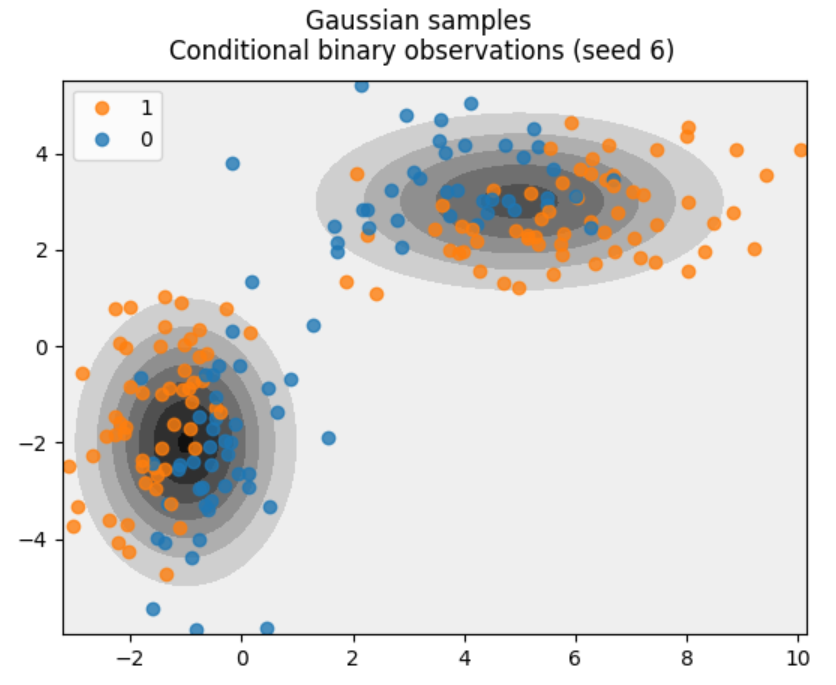
\includegraphics[scale=0.7]{images/samples_gmm_lc}
    \caption{Generated samples out of $K=2$ gaussians, labelized using a logistic model (label 1 or 0).
    The density of the hidden gaussians is represented in the background using shades of grey (black intense, white almost 0)}
    \label{fig:samples_gmm_lc}
\end{figure}

Note on the previous figure \ref{fig:samples_gmm_lc} that the limit between the labels in each subset gaussian is not sharp,
as it is sorted out of a probabilistic modelisation (logistic).
Consequently, an interesting observation can be made as we force the gaussians to have small values of mean and variance.
Indeed, as shown on the next figure, if we take the same parameters as previously and divide them by a factor 10,
the logistic model is ill conditioned.
\begin{figure}[H]
    \center
    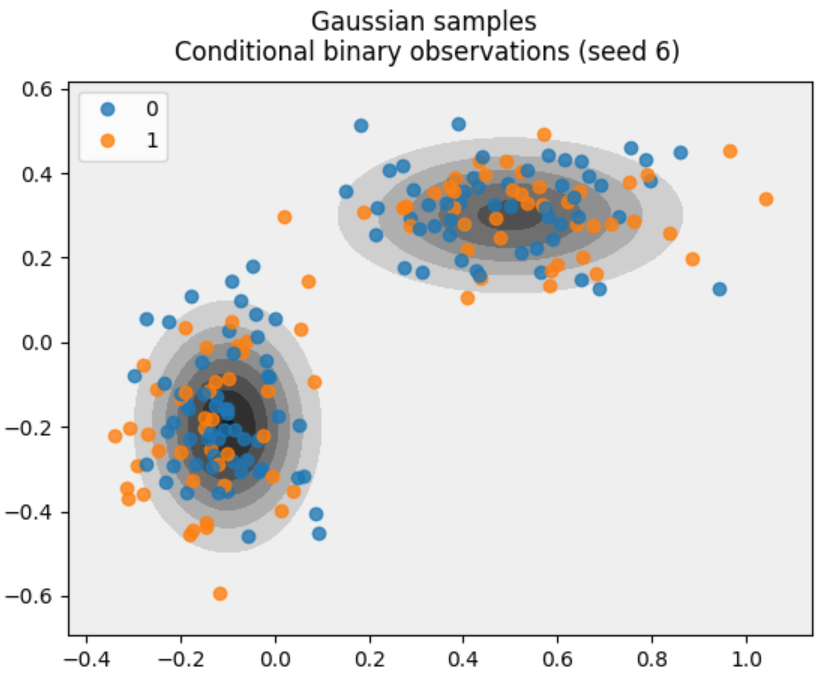
\includegraphics[scale=0.7]{images/samples_gmm_lc_badconditioning}
    \caption{Generated samples out of $K=2$ gaussians, using the same parameters as for figure \ref{fig:samples_gmm_lc} divided by a factor 10.}
    \label{fig:gmm_lc_badconditioning}
\end{figure}

All points are close to the frontier in terms of norm on figure \ref{fig:gmm_lc_badconditioning}.
Since we do not exploit any normalization term in the sigmoid modelization, this leads to a blurry area in which the linear separation model is not useful at all.
This situation is heavily problematic as it prevents us from performing a general benchmark on that dataset.
Indeed, the further larger the variance is, with sufficient samples, the better the linear approximation will be and therefore the better the modelization gets.
On the contrary, with smaller variance the linear model isn't descriptive of the generated samples as they are all close to the frontier, therefore with heavily noisy labelization.